% Template for a Computer Science Tripos Part II project dissertation
\documentclass[12pt,a4paper,twoside,openright]{report}
\usepackage[pdfborder={0 0 0}]{hyperref}    % turns references into hyperlinks
\usepackage[margin=25mm]{geometry}  % adjusts page layout
\usepackage{graphicx}  % allows inclusion of PDF, PNG and JPG images
\usepackage{verbatim}
\usepackage{docmute}   % only needed to allow inclusion of proposal.tex

\raggedbottom                           % try to avoid widows and orphans
\sloppy
\clubpenalty1000%
\widowpenalty1000%

\renewcommand{\baselinestretch}{1.1}    % adjust line spacing to make
                                        % more readable

\begin{document}

\bibliographystyle{plain}


%%%%%%%%%%%%%%%%%%%%%%%%%%%%%%%%%%%%%%%%%%%%%%%%%%%%%%%%%%%%%%%%%%%%%%%%
% Title


\pagestyle{empty}

\rightline{\LARGE \textbf{Martin Richards}}

\vspace*{60mm}
\begin{center}
\Huge
\textbf{How to write a dissertation in \LaTeX} \\[5mm]
Computer Science Tripos -- Part II \\[5mm]
St John's College \\[5mm]
\today  % today's date
\end{center}

%%%%%%%%%%%%%%%%%%%%%%%%%%%%%%%%%%%%%%%%%%%%%%%%%%%%%%%%%%%%%%%%%%%%%%%%%%%%%%
% Proforma, table of contents and list of figures

\pagestyle{plain}

\chapter*{Proforma}

{\large
\begin{tabular}{ll}
Name:               & \bf Martin Richards                       \\
College:            & \bf St John's College                     \\
Project Title:      & \bf How to write a dissertation in \LaTeX \\
Examination:        & \bf Computer Science Tripos -- Part II, July 2001  \\
Word Count:         & \bf 1587\footnotemark[1]
                      (well less than the 12000 limit)  \\
Project Originator: & Dr M.~Richards                    \\
Supervisor:         & Dr Markus Kuhn                    \\ 
\end{tabular}
}
\footnotetext[1]{This word count was computed
by \texttt{detex diss.tex | tr -cd '0-9A-Za-z $\tt\backslash$n' | wc -w}
}
\stepcounter{footnote}


\section*{Original Aims of the Project}

To write a demonstration dissertation\footnote{A normal footnote without the
complication of being in a table.} using \LaTeX\ to save
student's time when writing their own dissertations. The dissertation
should illustrate how to use the more common \LaTeX\ constructs. It
should include pictures and diagrams to show how these can be
incorporated into the dissertation.  It should contain the entire
\LaTeX\ source of the dissertation and the makefile.  It should
explain how to construct an MSDOS disk of the dissertation in
Postscript format that can be used by the book shop for printing, and,
finally, it should have the prescribed layout and format of a diploma
dissertation.


\section*{Work Completed}

All that has been completed appears in this dissertation.

\section*{Special Difficulties}

Learning how to incorporate encapulated postscript into a \LaTeX\
document on both Ubuntu Linux and OS X.
 
\newpage
\section*{Declaration}

I, [Name] of [College], being a candidate for Part II of the Computer
Science Tripos [or the Diploma in Computer Science], hereby declare
that this dissertation and the work described in it are my own work,
unaided except as may be specified below, and that the dissertation
does not contain material that has already been used to any substantial
extent for a comparable purpose.

\bigskip
\leftline{Signed [signature]}

\medskip
\leftline{Date [date]}

\tableofcontents

\listoffigures

\newpage
\section*{Acknowledgements}

This document owes much to an earlier version written by Simon Moore
\cite{Moore95}.  His help, encouragement and advice was greatly 
appreciated.

%%%%%%%%%%%%%%%%%%%%%%%%%%%%%%%%%%%%%%%%%%%%%%%%%%%%%%%%%%%%%%%%%%%%%%%
% now for the chapters

\pagestyle{headings}

\chapter{Introduction}

\section{Overview of the files}

This document consists of the following files:

\begin{itemize}
\item \texttt{makefile} --- The makefile for the dissertation and
                         Project Proposal
\item \texttt{diss.tex} --- The dissertation
\item \texttt{proposal.tex}  --- The project proposal 
\item \texttt{figs} -- A directory containing diagrams and pictures
\item \texttt{refs.bib} --- The bibliography database
\end{itemize}

\section{Building the document}

This document was produced using \LaTeXe which is based upon
\LaTeX\cite{Lamport86}.  To build the document you first need to
generate \texttt{diss.aux} which, amongst other things, contains the
references used.  This if done by executing the command:

\texttt{pdflatex diss}

\noindent
Then the bibliography can be generated from \texttt{refs.bib} using:

\texttt{bibtex diss}

\noindent
Finally, to ensure all the page numbering is correct run \texttt{pdflatex}
on \texttt{diss.tex} until the \texttt{.aux} files do not change.  This
usually takes 2 more runs.

\subsection{The makefile}

To simplify the calls to \texttt{pdflatex} and \texttt{bibtex}, 
a makefile has been provided, see Appendix~\ref{makefile}. 
It provides the following facilities:

\begin{description}

\item\texttt{make} \\
 Display help information.

\item\texttt{make proposal.pdf} \\
 Format the proposal document as a PDF.

\item\texttt{make view-proposal} \\
 Run \texttt{make proposal.pdf} and then display it with a Linux PDF viewer
 (preferably ``okular'', if that is not available fall back to ``evince'').

\item\texttt{make diss.pdf} \\
 Format the dissertation document as a PDF.

\item\texttt{make count} \\
Display an estimate of the word count.

\item\texttt{make all} \\
Construct \texttt{proposal.pdf} and \texttt{diss.pdf}.

\item\texttt{make pub} \\ Make \texttt{diss.pdf}
and place it in my \texttt{public\_html} directory.

\item\texttt{make clean} \\ Delete all intermediate files except the
source files and the resulting PDFs. All these deleted files can
be reconstructed by typing \texttt{make all}.

\end{description}


\section{Counting words}

An approximate word count of the body of the dissertation may be
obtained using:

\texttt{wc diss.tex}

\noindent
Alternatively, try something like:

\verb/detex diss.tex | tr -cd '0-9A-Z a-z\n' | wc -w/


\chapter{Preparation}

This chapter is empty!


\chapter{Implementation}

\section{Verbatim text}

Verbatim text can be included using \verb|\begin{verbatim}| and
\verb|\end{verbatim}|. I normally use a slightly smaller font and
often squeeze the lines a little closer together, as in:

{\renewcommand{\baselinestretch}{0.8}\small
\begin{verbatim}
GET "libhdr"
 
GLOBAL { count:200; all  }
 
LET try(ld, row, rd) BE TEST row=all
                        THEN count := count + 1
                        ELSE { LET poss = all & ~(ld | row | rd)
                               UNTIL poss=0 DO
                               { LET p = poss & -poss
                                 poss := poss - p
                                 try(ld+p << 1, row+p, rd+p >> 1)
                               }
                             }
LET start() = VALOF
{ all := 1
  FOR i = 1 TO 12 DO
  { count := 0
    try(0, 0, 0)
    writef("Number of solutions to %i2-queens is %i5*n", i, count)
    all := 2*all + 1
  }
  RESULTIS 0
}
\end{verbatim}
}

\section{Tables}

\begin{samepage}
Here is a simple example\footnote{A footnote} of a table.

\begin{center}
\begin{tabular}{l|c|r}
Left      & Centred & Right \\
Justified &         & Justified \\[3mm]
%\hline\\%[-2mm]
First     & A       & XXX \\
Second    & AA      & XX  \\
Last      & AAA     & X   \\
\end{tabular}
\end{center}

\noindent
There is another example table in the proforma.
\end{samepage}

\section{Simple diagrams}

Simple diagrams can be written directly in \LaTeX.  For example, see
figure~\ref{latexpic1} on page~\pageref{latexpic1} and see
figure~\ref{latexpic2} on page~\pageref{latexpic2}.

\begin{figure}
\setlength{\unitlength}{1mm}
\begin{center}
\begin{picture}(125,100)
\put(0,80){\framebox(50,10){AAA}}
\put(0,60){\framebox(50,10){BBB}}
\put(0,40){\framebox(50,10){CCC}}
\put(0,20){\framebox(50,10){DDD}}
\put(0,00){\framebox(50,10){EEE}}

\put(75,80){\framebox(50,10){XXX}}
\put(75,60){\framebox(50,10){YYY}}
\put(75,40){\framebox(50,10){ZZZ}}

\put(25,80){\vector(0,-1){10}}
\put(25,60){\vector(0,-1){10}}
\put(25,50){\vector(0,1){10}}
\put(25,40){\vector(0,-1){10}}
\put(25,20){\vector(0,-1){10}}

\put(100,80){\vector(0,-1){10}}
\put(100,70){\vector(0,1){10}}
\put(100,60){\vector(0,-1){10}}
\put(100,50){\vector(0,1){10}}

\put(50,65){\vector(1,0){25}}
\put(75,65){\vector(-1,0){25}}
\end{picture}
\end{center}
\caption{A picture composed of boxes and vectors.}
\label{latexpic1}
\end{figure}

\begin{figure}
\setlength{\unitlength}{1mm}
\begin{center}

\begin{picture}(100,70)
\put(47,65){\circle{10}}
\put(45,64){abc}

\put(37,45){\circle{10}}
\put(37,51){\line(1,1){7}}
\put(35,44){def}

\put(57,25){\circle{10}}
\put(57,31){\line(-1,3){9}}
\put(57,31){\line(-3,2){15}}
\put(55,24){ghi}

\put(32,0){\framebox(10,10){A}}
\put(52,0){\framebox(10,10){B}}
\put(37,12){\line(0,1){26}}
\put(37,12){\line(2,1){15}}
\put(57,12){\line(0,2){6}}
\end{picture}

\end{center}
\caption{A diagram composed of circles, lines and boxes.}
\label{latexpic2}
\end{figure}



\section{Adding more complicated graphics}

The use of \LaTeX\ format can be tedious and it is often better to use
encapsulated postscript (EPS) or PDF to represent complicated graphics.
Figure~\ref{epsfig} and~\ref{xfig} on page \pageref{xfig} are
examples. The second figure was drawn using \texttt{xfig} and exported in
{\tt.eps} format. This is my recommended way of drawing all diagrams.


\begin{figure}[tbh]
\centerline{
\includegraphics{figs/cuarms.pdf}}
\caption{Example figure using encapsulated postscript}
\label{epsfig}
\end{figure}

\begin{figure}[tbh]
\vspace{4in}
\caption{Example figure where a picture can be pasted in}
\label{pastedfig}
\end{figure}


\begin{figure}[tbh]
\centerline{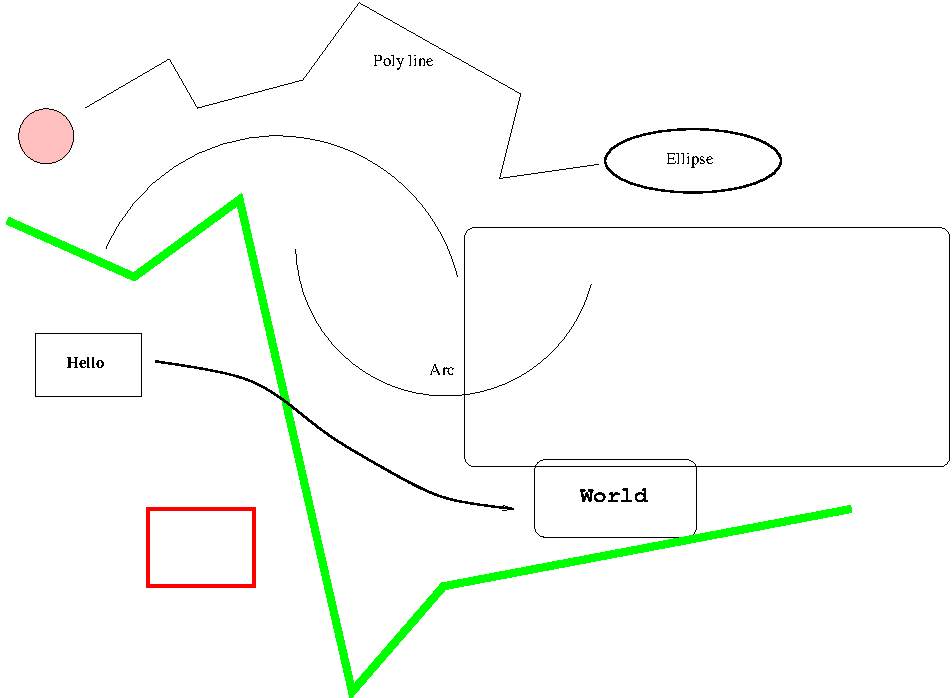
\includegraphics{figs/diagram.pdf}}
\caption{Example diagram drawn using \texttt{xfig}}
\label{xfig}
\end{figure}


\chapter{Evaluation}

\section{Printing and binding}

Use a ``duplex'' laser printer that can print on both sides to print
two copies of your dissertation. Then bind them, for example using the
comb binder in the Computer Laboratory Library.

\section{Further information}

See the Unix Tools notes at

\url{http://www.cl.cam.ac.uk/teaching/current-1/UnixTools/materials.html}


\chapter{Conclusion}

I hope that this rough guide to writing a dissertation is \LaTeX\ has
been helpful and saved you time.


%%%%%%%%%%%%%%%%%%%%%%%%%%%%%%%%%%%%%%%%%%%%%%%%%%%%%%%%%%%%%%%%%%%%%
% the bibliography
\addcontentsline{toc}{chapter}{Bibliography}
\bibliography{refs}

%%%%%%%%%%%%%%%%%%%%%%%%%%%%%%%%%%%%%%%%%%%%%%%%%%%%%%%%%%%%%%%%%%%%%
% the appendices
\appendix

\chapter{Latex source}

\section{diss.tex}
{\scriptsize\verbatiminput{diss.tex}}

\section{proposal.tex}
{\scriptsize\verbatiminput{proposal.tex}}

\chapter{Makefile}

\section{makefile}\label{makefile}
{\scriptsize\verbatiminput{makefile.txt}}

\section{refs.bib}
{\scriptsize\verbatiminput{refs.bib}}


\chapter{Project Proposal}

% Note: this file can be compiled on its own, but is also included by
% diss.tex (using the docmute.sty package to ignore the preamble)
\documentclass[12pt,a4paper,twoside]{article}
\usepackage[pdfborder={0 0 0}]{hyperref}
\usepackage[margin=25mm]{geometry}
\usepackage{graphicx}
\usepackage{parskip}
\begin{document}

\begin{center}
\Large
Computer Science Tripos -- Part II -- Project Proposal\\[4mm]
\LARGE
Brain tumour segmentation using Convolutional Neural Networks

\large
S.~Borgeaud~dit~Avocat, Fitzwilliam College

Originator: D.~Wang

11 October 2016
\end{center}

\vspace{5mm}

\textbf{Project Supervisor:} Dr M.~Jamnik \& D.~Wang

\textbf{Director of Studies:} Dr R.~K.~Harle

\textbf{Project Overseers:} Prof J.~Bacon  \& Prof R.~Anderson

% Main document

\section*{Introduction}

Over the last years deep learning, more specifically convolutional neural networks (CNN), have outperformed other machine learning techniques in many tasks such as image classification \cite{nature-deep-learning-review}. The field of bioinformatics is no exception to this, in particular, convolutional neural networks have been shown to perform as well as previous state-of-the-art algorithms on the problem of brain tumour segmentation \cite{brats-proceedings}.

The aim of this project is to use convolutional neural networks to replicate these recent results on the brain tumour segmentation problem. This project will concentrate exclusively on the dataset provided by the BraTS2013\footnote{\url{http://martinos.org/qtim/miccai2013/}} grand challenge on which many different algorithms have already been tested and will provide a good framework to test and compare my work.

As a starting point I will follow the paper written by Pereira et al \cite{pereira}. The approach used is to cut the magnetic resonance images into multiple patches and regard the problem as a classification problem of the pixel located at the center of the patch. The aim is to classify each pixel into one of these four classes:
\begin{enumerate}
	\item Non-tumor
	\item Surrounding edema
	\item Non-enhancing tumour
	\item Enhancing tumour
\end{enumerate}
\section*{Starting point}
  
The starting point for this project is the part 1B course 'Artificial Intelligence 1'  which provided a short introduction to machine learning. In particular multi-layer perceptrons, the sigmoid activation function, backpropagation and stochastic gradient descent training were introduced. These concepts are all reused in convolutional neural networks which add convolutional and pooling layers to conventional multi-layer perceptrons network.

I will be using the Keras library with Tensor Flow to create and train convolutional neural networks.

Keras is a library written for Python. Fortunately, I have used Python before in small side projects meaning that I won't have to spend time learning a new language.

As the problem is self contained and formulated purely as a a machine learning task, none or very little biological/medical background knowledge is required.

\section*{Resources required}

For this project I will mainly use my own quad-core computer which
runs Mac OS X El Capitan. I accept full responsibility for this machine and I have made contingency plans to protect myself against hardware and/or software failure. In case of failure, I will be able to terminate my project using the MCS machines.  Backups will be to my external hard disk. Once a week, I will also copy all files to my Google Drive to add an extra level of redundancy in case of hardware failure. All written code will be under version control using git and will be backed up on a private GitHub repository at least daily while working on it. 

I will also need a computer with an external GPU to train the neural network in a reasonable amount of time. For this, I will be using the Cambridge High Performance cluster. Alternatively, if this is not possible, I will use a GPU that would be provided by the AI group.

\section*{Work to be done}

The project breaks down into the following phases:

\begin{enumerate}

\item The first phase of the project will be mainly focused on research during which I will learn how convolutional networks  work and read up on how they have been used on the brain tumour segmentation problem in different papers. I plan to complete the Stanford CS321n\footnote{\url{http://cs231n.github.io/}} course on convolutional neural networks that I have already started. I will also need to learn how to use the Keras and TensorFlow libraries and review some of the more advanced Python features that I haven't used recently.

\item The second phase will mainly be devoted to preparing the images obtained from the BRATS dataset. The images will need to be cut into patches each of which will have to be normalised. I will need to perform bias field correction as magnetic resonance images can exhibit non-uniformities that are the result of magnetic field variations rather than anatomical differences \footnote{\url{http://brainsuite.org/processing/surfaceextraction/bfc/}}. I will then need to perform intensity normalisation across the different images. Finally, I will need to add the correct label to each patch using the segmentation provided with the original training images.

\item The next step will be to use the prepared and normalised patches to train a convolutional neural network using the Keras library. This will require hyperparameter tuning using cross-validation to avoid overfitting. I will then construct segmented images using my convolutional neural network to delimit the different segments to get a visual result that is easy to interpret.

\item During the last step I will evaluate how well my convolutional neural network performed using standard methods used to evaluate classifiers such as the confusion matrix, recall, precision and Dice scores. This evaluation can be done for different hyperparameters. Because the dataset has been used many times before as part of the Grand Challenge\footnote{\url{https://grand-challenge.org}} I will also be able to perform a quantitative comparison with different segmentation algorithms also using convolutional neural networks as well as other algorithms using different techniques.

\end{enumerate}

\section*{Success criteria}

The main success criteria for this project will be to have an algorithm that performs brain tumour segmentation into the 4 different segments as discussed earlier. 

The primary aim is to achieve similar results to those obtained by Pereira et al \cite{pereira}, hopefully achieving 90\% of the accuracies obtained in the paper. This means achieving the Dice\footnote{\url{https://en.wikipedia.org/wiki/Sorensen-Dice\_coefficient}} scores summarised in the following table, where `complete' refers to the complete tumour region (including classes 2--4), `core' refers to all regions except for the edema structure (classes 3--4) and `enhancing' includes only the enhancing tumour (class 4):

\begin{center}
\begin{tabular}{ |c|c|c| } 
\hline
complete & core & enhancing \\
\hline
 0.79 & 0.74 & 0.69  \\ 
\hline
\end{tabular}
\end{center}



\section*{Possible extensions}

Due to the recent development of this area, this project naturally leads to multiple possible extensions:
\begin{enumerate}
	\item This process of segmenting MRI scans is very slow as each scan has to be cut into patches, one per pixel, and each patch then needs to be classified. Recent techniques have shown that it is possible to classify all pixels of a patch at once, which would drastically improve the speed of the segmentation. A possible extension would be to try to improve the segmentation speed using the suggested technique. It would then be interesting to compare the performance of the faster algorithm to the performance of the original one.
	\item Experiment with the layout of the neural network, in particular change the number of layers and the type of the layers of the convolutional neural network to try to improve the accuracy.
	\item Instead of using the Keras library, implement similar functionality myself using TensorFlow. I could then compare the results obtained by my implemention with those obtained using Keras. This will show and require a deeper understanding of how convolutional neural networks work.
	\item Use different data prepocessing/normalisation techniques and analyse how they affect the final accuracy of the convolutional neural network.
	\item Apply more recent techniques used to improve convolutional neural networks such as Dropout \cite{dropout}, Maxout \cite{maxout} or Batch Normalization \cite{batch_normalization} in order to improve the accuracy of the classification.
\end{enumerate}

\section*{Timetable}

Planned starting date is 21/10/2016.

\subsection*{Michaelmas term}
\begin{enumerate}
\item \textbf{Weeks 3--4} Learn about Convolutional Neural Networks by finishing the CS321n online course. Read papers about using Convolutional Neural Networks for brain tumour segmentation.

\emph{Milestone:} Understand the theory behind convolutional neural networks and be familiar with some of the more recent applications of them on the brain tumour segmentation problem.

\item \textbf{Weeks 5--6} Become familiar with the Keras library and refresh my Python knowledge. Download and play with the dataset.

\emph{Milestone:} Be comfortable enough with Keras and Python to be able to start the main part of the project.

\item \textbf{Weeks 7--8} Prepare the dataset for the implementation of the convolutional neural network. This includes performing the different normalisations.

{Milestone:} Have the dataset ready, that is split up into normalised patches. Each patch should have the corresponding label for the pixel that is located at its center.

\item \textbf{Christmas Vacation} Implement and train a convolutional neural network and perform the necessary cross-validation on the different hyperparameters. Create segmented brain images using my classifier.

{Milestone:} Have a working convolutional neural network that is able to classify the different patches with the required accuracy mentioned in the primary success criteria. Have some images that are segmented using the trained classifier.
\end{enumerate}


\subsection*{Lent term}
\begin{enumerate}

\item \textbf{Weeks 1--3} Write the progress report and prepare the presentation.

{Milestone:} Have the progress report submitted on time and be ready to give the presentation.

\item \textbf{Weeks 4--5} Evaluate the performance of my segmentation algorithm and look for possible improvements.

{Milestone:} Have the evaluation data of my convolutional neural network.

\item \textbf{Weeks 6--8} Compare the performance of my algorithm with the benchmarks available online and implement some of the extensions if time permits.

{Milestone:} Have all the necessary data for the final evaluation of my project.

\item \textbf{Easter Vacation} Write the main chapters of the dissertation. Implement some of the extensions if time permits.

{Milestone:} Have a complete first draft of my dissertation

\end{enumerate}

\subsection*{Easter term}
\begin{enumerate}
\item \textbf{Weeks 1--2} Improve the dissertation where necessary

{Milestone:} Have the dissertation in its final form
\item \textbf{Weeks 3--4} Proof read the dissertation and submit it.

{Milestone:} Have the dissertation submitted.

\end{enumerate}

\end{document}

\end{document}
